\documentclass{standalone}
%This image was created by [Jake](http://tex.stackexchange.com/users/2552/jake) ([source](http://tex.stackexchange.com/a/118573/5645))
\usepackage{pgfplots}
\pgfplotsset{compat=1.9}
\begin{document}

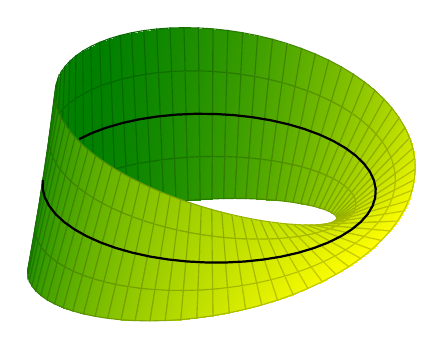
\begin{tikzpicture}
\begin{axis}[
    hide axis,
    view={40}{40}
]
\addplot3 [
    surf, shader=faceted interp,
    point meta=x,
    colormap/greenyellow,
    samples=80,
    samples y=5,
    z buffer=sort,
    domain=0:360,
    y domain=-0.5:0.5
] (
    {(1+0.5*y*cos(x/2)))*cos(x)},
    {(1+0.5*y*cos(x/2)))*sin(x)},
    {0.5*y*sin(x/2)});

\addplot3 [
    samples=50,
    domain=-145:180, % The domain needs to be adjusted manually, depending on the camera angle, unfortunately
    samples y=0,
    thick
] (
    {cos(x)},
    {sin(x)},
    {0});
\end{axis}
\end{tikzpicture}
\end{document}
